\documentclass[11pt,twoside,lineno]{GSA_format}
% Use the documentclass option 'lineno' to view line numbers
\usepackage[normalem]{ulem}
\useunder{\uline}{\ul}{}
\articletype{inv} % article type

\newcommand{\bm}[1]{\mbox{\boldmath{$#1$}}}

\title{A window-based approach to incorporating information from linked sites in genotype-environment association studies}

\author[$\ast$]{Tom R. Booker}
\author[$\dagger$]{Samuel Yeaman}
\author[$\ast$]{Michael C. Whitlock}

\affil[$\ast$]{University of British Columbia}
\affil[$\dagger$]{University of Calgary}

\keywords{Local Adaptation, Population Genetics, Environmental Genomics}

\runningtitle{Incorporating linkage in GEA analyses} % For use in the footer 

\runningauthor{Booker \textit{et al.}}

\begin{abstract}
\textit{I'm just using the GENETICS template because it looks nice!}

Here is a really concise and nicely written summary of the paper, highlighting the main findings and take home messages. \\



\end{abstract}

\begin{document}

\maketitle
%\thispagestyle{firststyle}
\marginmark
\firstpagefootnote


%\correspondingauthoraffiliation{1}{Corresponding author: booker@zoology.ubc.ca}
\vspace{-33pt}% Only used for adjusting extra space in the left column of the first page

\section{Introduction}

With an understanding of the genes or genomic regions involved in adaptation, we might work towards conservation programs. Furthermore, developing our understanding of the genetic architecture of adaptation may help us inform models of the limits and constraints of evolvability. 
Paragraph on local adaptation and why we might want to find the genes involved. \\

Theoretical studies of local adaptation suggest that we should expect regions of the genome subject to spatially varying selection pressures to exhibit elevated linkage disequilibrium relative to the genomic background. There are several possible reasons why this might be the case. Firstly, a locus subject to strong spatially varying selection can act as a barrier to gene flow in that particular region of the genome and generate LD with neutrally evolving sites in surrounding regions (Barton and Bengston et al). Secondly, there is a selective advantage for alleles that are involved in local adaptation to aggregate in regions of low recombination so favourable combinations of alleles may be bound together into regions of high LD (Rieseberg 2001; Noor et al 2001; Kirkpatrick and Barton 2006; Yeaman 2012). For example, in sunflowers and \textit{Littorina} marine snails there is evidence that regions of suppressed recombination cause alleles involved in local adaptation to be inherited together (Morales et al 2019; Todesco et al 2020) and in conifers many of the genes putatively involved in local adaptation are in LD with each other (Yeaman et al 2016). Of course, the two processes we have outlined are not mutually exclusive, but overall genomic regions containing strongly selected alleles that contribute to local adaptation will potentially exhibit signals expected under local adaptation at multiple linked sites. \\

A signature of local adaptation that can potentially be identified through the analysis of population genomic data is a correlation between allele frequencies and putatively selective features of the environment. So-called genotype-environment association (GEA) studies calculate and contrast such a correlation for many markers (typically single nucleotide polymorphisms, hereafter SNPs) across the genome. The strength of evidence for a particular SNP may be measured using \emph{p}-values, \emph{q}-values or Bayes factors. Genomic regions with particularly strong evidence for correlation with the environment may then indicate the presence of alleles that contribute to local adaptation. \\

In the context of GEA, the term environment may refer to any abiotic or biotic variable that the species of interest could conceivably be adapting/adapted to. Species distributed over space may inhabit a wide variety of environments, but these could potentially be correlated with demography. For example, many environmental variables would be strongly correlated with latitude or longitude, so species that inhabit North-South ranges, may exhibit a correlation with many environmental variables due to population demography alone. Attempts to identify genomic loci involved in adaptation may then be stymied by an underlying correlation between presumed selection gradients and directions of gene flow; Sohail et al (2018) and Berg et al (2018) provide a clear example of this problem in an analysis of selection on human height. For that reason, GEA methods may correct for population demography when calculating correlations with the environment. For example, the commonly used BayEnv and BayPass packages estimate a population covariance matrix from SNP data, then use it as a fixed parameter when estimating correlations between the frequencies of individual SNPs and the environment. 

Linked sites do not evolve independently. If the rate of recombination is low relative to the rate of migration, there may be strong autocorrelation in the coalescent histories among tightly linked sites. Under that assumption, all of the neutral SNPs present within an appropriately sized region provide independent tests of the following hypothesis, "is the genetic variation in this genomic region associated with variation in the environment?".




using combining information across tightly linked sites to identify regions of the genome under selection. 
Typically GEA studies examine patterns of genetic variation across a landscape at many polymorphic sites.  

\section{Materials and Methods}
\label{sec:materials:methods}

\subsection{\underline{The Weighted-Z Analysis}} 

In this study, we propose the Weighted-Z Analysis (hereafter, the WZA) for combining information across linked sites in the context of GEA studies. The weighted-Z test combines \textit{p}-values from multiple independent tests into a single score with each test given a weight that is proportional to the inverse of its error variance (Whitlock 2004). Inspired by Weir and Cockerham's (1984) method for combining estimates of $F_{ST}$ across sites, we use a marker's allele frequency to determine weights when performing the Weighted-Z test on GEA data. At a given polymorphic site, we denote the average frequency of the minor allele across populations as $\overline{p}$ ($\overline{q}$ corresponds to the major allele). The product $\overline{p}\overline{q}$ provides an estimate of the variance in allele frequencies among populations, so is appropriate as a weight.

We combine information from multiple GEA tests performed on SNPs present in a particular region into a single weighted-Z score ($Z_W$). For genomic region \textit{k}, which contains \textit{n} polymorphic sites, we calculate 

\begin{equation}
\label{weightedZ}
Z_{w,k} =  \frac {\sum\limits_{i=1}^n \overline{p_i} \overline{q_i}z_i}{\sqrt{ \sum\limits_{i=1}^n (\overline{p_i}\overline{q_i})^2} },
\end{equation}
where $\overline{p_i}$ and $\overline{q_i}$ are the average allele frequencies across demes for polymorphism \textit{i} and $z_i$ is the standard normal deviate calculated from the one-side \textit{p}-value for SNP \textit{i}.



\subsection{\underline{The top-candidate test}} 

Yeaman et al (2016) proposed a method for combining information across sites in genotype-environment association studies. The top-candidate test, as Yeaman et al (2016)  called it, attempts to identify regions of the genome involved in local adaptation under the assumption that alleles in such regions will tend to generate LD with neighbouring sites so multiple linked markers may exhibit a significant correlation with important environmental variables. First, the genome-wide distribution of SNPs is examined to identify outliers. SNPs with \textit{p}-values above a particular percentile threshold genome-wide (we used the 99th percentile) are classified as outliers. The frequency of outliers SNPs in analysis windows is then compared to the total number of SNPs in the window. A binomial test is used to determine whether a given window has an excess of outliers relative to the genome-wide expectation. Analysis windows with a \textit{p}-value less than 0.0001 were taken as "top-candidates" for local adaptation. Note that in Yeaman et al (2016) genes, as well as up and downstream flanking sequence, were used as analysis windows. 


\subsection{\underline{Simulating local adaptation}} 

Genotype-environment association studies are often performed on large spatially extended populations. However, it is computationally infeasible to model selection and linkage in large chromosome in such a populations, so we scaled population genetic parameters to tractably model large populations. Table \ref{SimulationParameters} shows the parameters of the organism that we evolved \textit{in silico}. In the Appendix, we outline and justify the approach we used to scale relevant population genetic parameters in our simulations of local adaptation. All simulations were performed in SLiM v3.4 (Messer and Haller 2018). \\
 
We simulated genomes with a single chromosome containing 1,000 "genes". Each "gene" was 9,999bp long and recombined at a rate of $r = 10^{-7}$, between each gene a single base-pair recombined at a rate of $r = 0.005$. Thus, our simulated chromosomes were 10Mbp long each, but modelled a 599 cM chromosome. \\

The simulated populations inhabited a $14\times14$ 2-dimensional stepping-stone population.

%Local adaptation can act as a barrier to gene-flow, individuals that migrate from locations where they are well adapted into locations where they are disfavoured may not survive to propagate, so even freely recombining regions of the genome are linked to a degree and will influence evolution in regions of the genome that are freely recombining. To model local adaptation in unlinked regions of the genome, we modelled three cartoon chromosomes. The cartoon chromosomes were short sequences, 1,000bp long, that had a genetic map and net mutation rate (\textit{$U_a$}) that was the as the focal chromosome. 

We simulated three kinds of environment. The first was a reduced representation of climatic variation across British Columbia, Canada. We downloaded the map of degree days greater than 0 (DD0) for British Columbia from ClimateBC (website; REF). From the DD0 map (Figure 1A), we extracted the data for a 99x99 grid using Dog Mountain, BC as the reference point in the South-West corner. We divided this map into a 14x14 grid. Each cell corresponded to an area of XX$km^2$. We calculated the mean DD0 for each cell in the grid. We then converted the mean DD0 scores into Z-scores and rounded values up to the nearest third. These data were then used as the phenotypic optima for population models in SLiM. The data from the BC Map were then ordered along one axis of the 2D stepping-stone, we refer to this map as the \textit{cline} map (Figure 1C). Finally, we truncated the distribution of Z-scores from the BC map at +3, setting all demes with a DD0 Z score greater than or equal to 3 to 3, and all others to -1. We refer to this map as the \textit{Truncated map} (Figure 1D).

In addition, we simulated local adaptation in a metapopultion with no spatial structure (i.e. an island model).  The first is the island model, which represents an unstructured metapopulation. 

%We constructed a map using data for real climate variation from British Columbia, Canada. We downloaded the map of degree days greater than 0 for British Columbia from ClimateBC (website; REF). From the DD0 map, we extracted the data for a 99x99 grid using Dog Mountain, BC as the reference point in the South-West corner. We divided this map into a 16x16 grid and calculated the mean DD0 for each cell. We converted the means into Z-scores and rounded values up to the nearest third of a Z-score. These data were then used as the phenotypic optima for a structured population models in SLiM.

%We simulated local adaptation using a model of stabilising selection. We modelled a genome of composed of four autosomes. 

%We used the standard expression for Gaussian stabilising selection,
%\begin{equation}
%\notag
%W(z_{i,j}) = exp \Big[\frac{-(z_{i,j} - \theta_j)^2}{2V_s}\Big],
%\end{equation}
%where $z_i$ is the phenotype of the $i^{th}$ individual in environment $j$, $\theta_j$ is the phenotypic optimum of environment $j$, and $V_s$ is the variance of the Gaussian fitness function. 

To test the performance of the weighted-Z analysis (WZA), we modelled populations adapting to various environments. Figure \ref{fig:EnvGrid} shows a diagram of each of the populations simulated.


\subsection{Covariance of phenotype and environment} 

In our simulations modelling stabilising selection, we used the covariance between phenotypes and environment as a measure of a gene's relevance for local adaptation. We calculated the average phenotypic effect of each gene as follows.
We then used Cov($PB_g$, $env$)/Cov($PB$, $env$) as a measure of a gene's contribution to local adaptation.


In our simulations, phenotypic variance ($\sigma^{2}_{P}$) was generated solely by genotypes, i.e. there were no environmental effects. Local adaptation generates variance in phenotypes between populations ($\sigma^{2}_{PB}$). 
As described above, the simulations incorporated a stochastic mutation model, so from replicate to replicate the effect size of alleles and their locations in the genome varied. As a result, the genes that contributed to local adaptation varied across simulation replicates. We therefore determined the contribution  each gene made to local adaptation by calculating the proportion of phenotypic variance among populations explained by the SNPs in each gene. For each gene that contributes to phenotypic variation there are $k$ causal SNPs each with a phenotypic effect of $\alpha_k$. We use $\bm{\nu_g}$ to refer to the column vector of phenotypic effects for each of the $k$ causal SNPs in gene $g$. In each population there are $n$ diploid individuals and we have $\bm{M_d}$, an $n \times k$ matrix in which the genotype of each individual at each causal SNP is coded as 0, 1 or 2 corresponding to aa, aA and AA genotypes, respectively. The contribution that each gene makes to the overall phenotype in each population is calculated as $C_{g,d} = \sum \bm{M_{g,d} \nu_{g,d}}$. The variance in $C_{g,d}$ gives us a measure of the phenotypic variance between popuatlions generated by each gene ($\sigma^{2}_{PB,g}$). We then calculate the proportion of variance explained by each gene ($PVE_g$) as $\sigma^{2}_{PB,g} / \sigma^{2}_{PB}$
\begin{equation}
PVE_g = \frac{\sigma^{2}_{PB,g}}{\sigma^{2}_{PB}}.
\end{equation}

Note that $PVE_g$ does not provide a measure of local adaptation, merely a measure of how much phenotypic variation between populations can be explained by a a particular gene. 
For each of the 50 genes in a simulated chromosome, we recorded the $PVE$ for QTL and for non-QTL the distance to the 

\subsection{Analysis of simulation data}

We added neutral mutations to each simulated tree sequence at a rate of $1\times10^{-8}$ using PySLiM (version). While this gave us a population scaled mutation rate of $4N_ed\mu = 0.00078$, and resulted in an average of 30 SNPs per gene that passed a minor allele frequency filter of 0.05.

For each SNP, we calculated Kendall's $\tau$ and recorded the $p$-value. We chose Kendall's $\tau$ over Spearman's $\rho$ as an uncorrected GEA statistic as it can handle ties in data, 


\subsection{Analysis of data from Lodgepole pine}

We re-analysed a population genomic dataset collected for lodgepole pine distributed across the North West of North America. The data were initially generated and described by Yeaman et al (2016). Initially, the top-candidate test was applied to this data. We calculated $Z_W$ scores for the same genes analysed by Yeaman et al (2016). Data were accessed from the Dryad respository associated with Yeaman et al (2016) (DRYADLINK)

\subsection{Data Availability}

The simulation configuration files and code to perform the analysis of simulated data and generate the associated plots are available at github/TBooker/GEA. Tree-sequence files for the simulated populations are available at Dryad and all processed GEA files are available on (https://doi.org/10.5061/dryad.0t407). 

%%%%%%%%% %
%       % %
%       % %
%       % %
%%%%%%%%% %
%  %
%   %
%    %
%     %
%      %
\section{Results}

\subsection{Statistical properties of the WZA}

To assess the statistical properties of the WZA and the top-candidate test, we first performed GEA analyses on populations structured according to an island model. While highly unrealistic, analysing this model allowed us to determine the statistical properties of the WZA and the top-candidate test without the need to correct for the confounding effects of population structure. 

The distribution of $Z_W$ scores obtained for populations evolving under strict neutrality was very close to the expectation of the standard normal distribution. The mean $Z_W$ was 0.00X and the variance was 1.XXX. Figure \ref{fig:normalIsland}A shows the distribution of $Z_W$ scores obtained when analysing a sample consisting of 50 individuals from 40 demes (2,000 total).  However, simulations modelling local adaptation in the island model resulted in a skewed distribution of $Z_W$ scores for neutral genes. Figure \ref{fig:normalIsland}C shows that adaptation elsewhere in the genome can generate a background level of correlation with the environment, causing the mean $Z_W$ to be greater than 0. Indeed, the mean $Z_W$ was 0.00X and the variance was 1.XXX in this case. This isolation-by-adaptation means that it is not possible to convert $Z_W$ scores to parametric \textit{p}-values. 
Some degree of isolation-by-adaptation should probably be expected in natural organisms

The populations we simulated had \textbf{5} chromosomes, one of which was strictly neutral. Applying the WZA to simulated genes from a neutrally evolving chromosome in a locally adaptated population allows us to test whether isolation-by-adaptation causes a 

\begin{figure}
  \includegraphics[width=\linewidth]{../../Plots/environmentGridPlot_2x2.png}
  \caption{Three models of population structure used to simulated varying degrees of spatial autocorrelation in the environment. A) A highly discretized map of degree-days above 0 (DD0) in South-Western British Columbia, capturing realistic spatial autocorrelation in an environmental variable species may respond to. We refer to the map in A as the BC map. B) A 1-dimensional cline in phenotypic optimum, we refer to this as the cline map. C) A heterogenous distribution of phenotyic optima. The distribution of phenotypic optima in the cline and random maps}
  
  \label{fig:boat1}
\end{figure}

\subsection{Comparison of the WZA and the top-candidate test}



\begin{figure}
  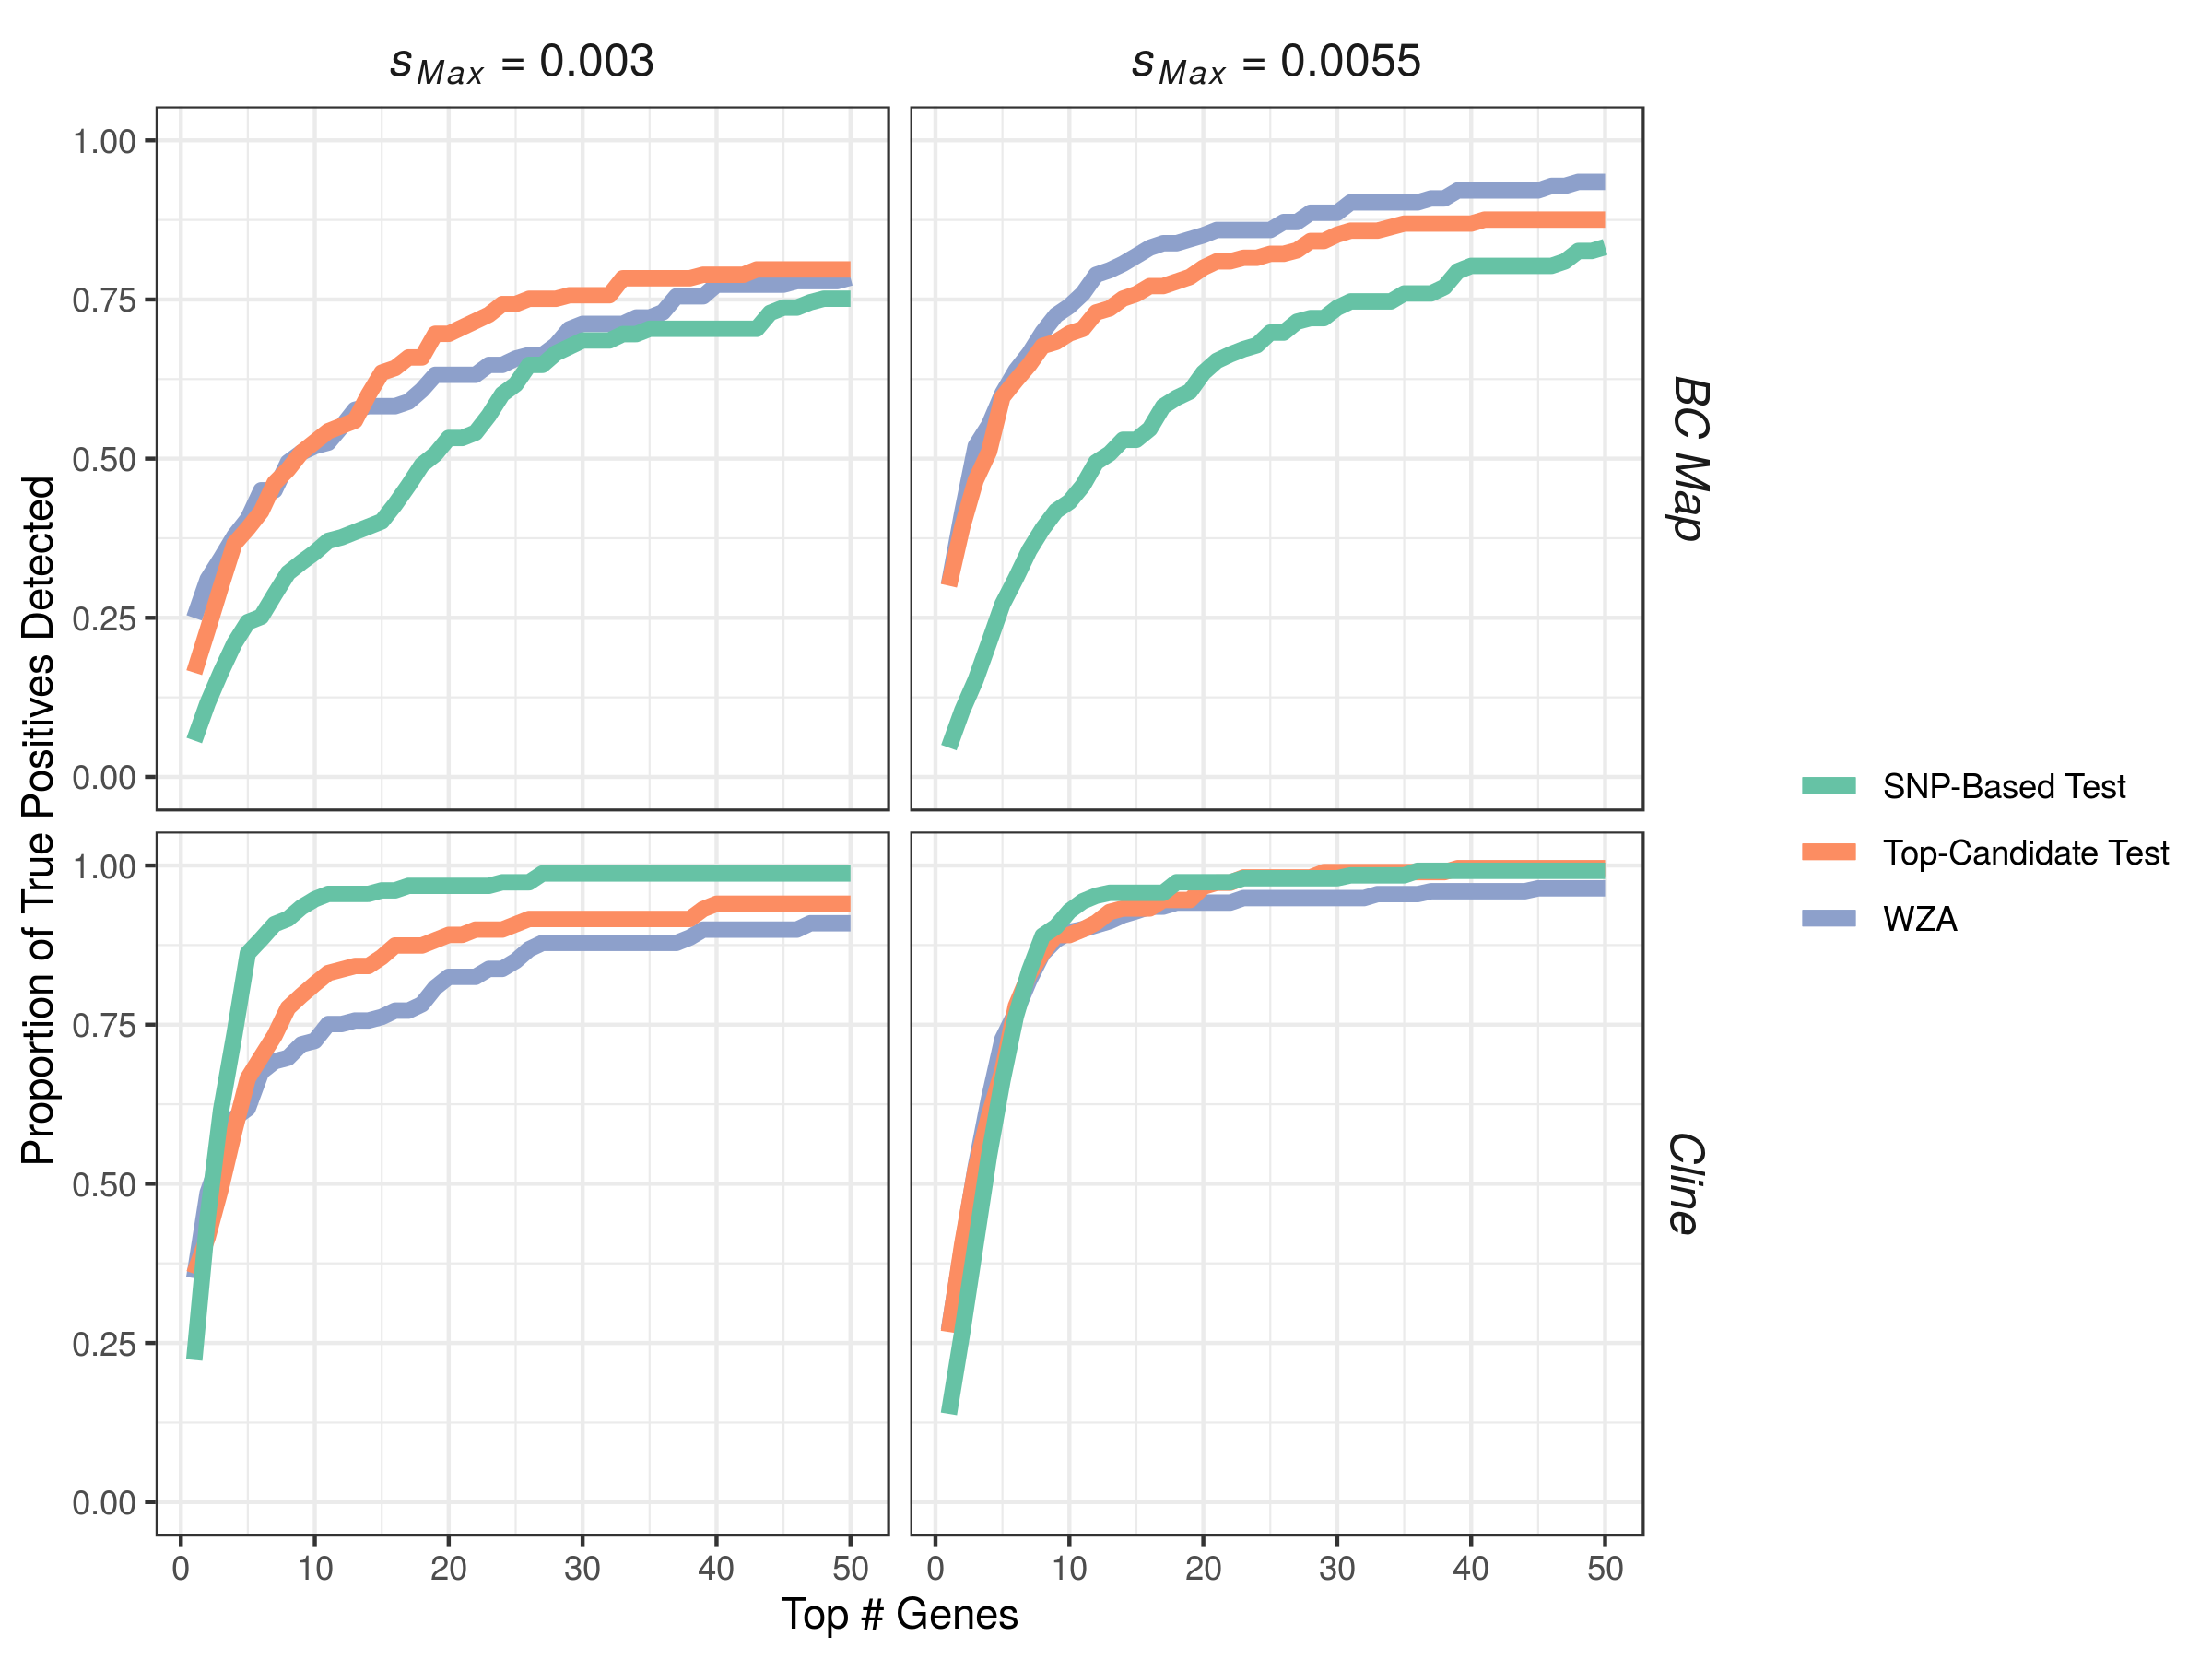
\includegraphics[]{../SimulationStudy/directionalSelection/G.2.3/PowerPlot_sampledData.png}
  \caption{Summary statistics from simulations. A) shows the $F_{ST}$ between pairs of demes in stepping-stone populations, the average across replicates is . B) shows the average LD between pairs of SNPs, each line corresponds to a single simulation replicate.}

  \label{fig:lodgepole}
\end{figure}


\subsection{Recombination rate variation}

Recombination rates vary widely among taxa but also within the genome (Stapley et al REVIEW). 

\subsection{Application of the WZA to data from lodgepole pine}

To demonstrate how one might apply the WZA to the analysis of real data, we re-analysed the lodgepole pine (\textit{Pinus contorta}) data from Yeaman et al (2016). Briefly, Yeaman et al (2016) collected samples from 666 populations across British Columbia and Alberta, Canada and from Northern Washington, USA. Individuals in each 
Data were downloaded from the Dryad repository associated with the paper. 

\begin{figure}
  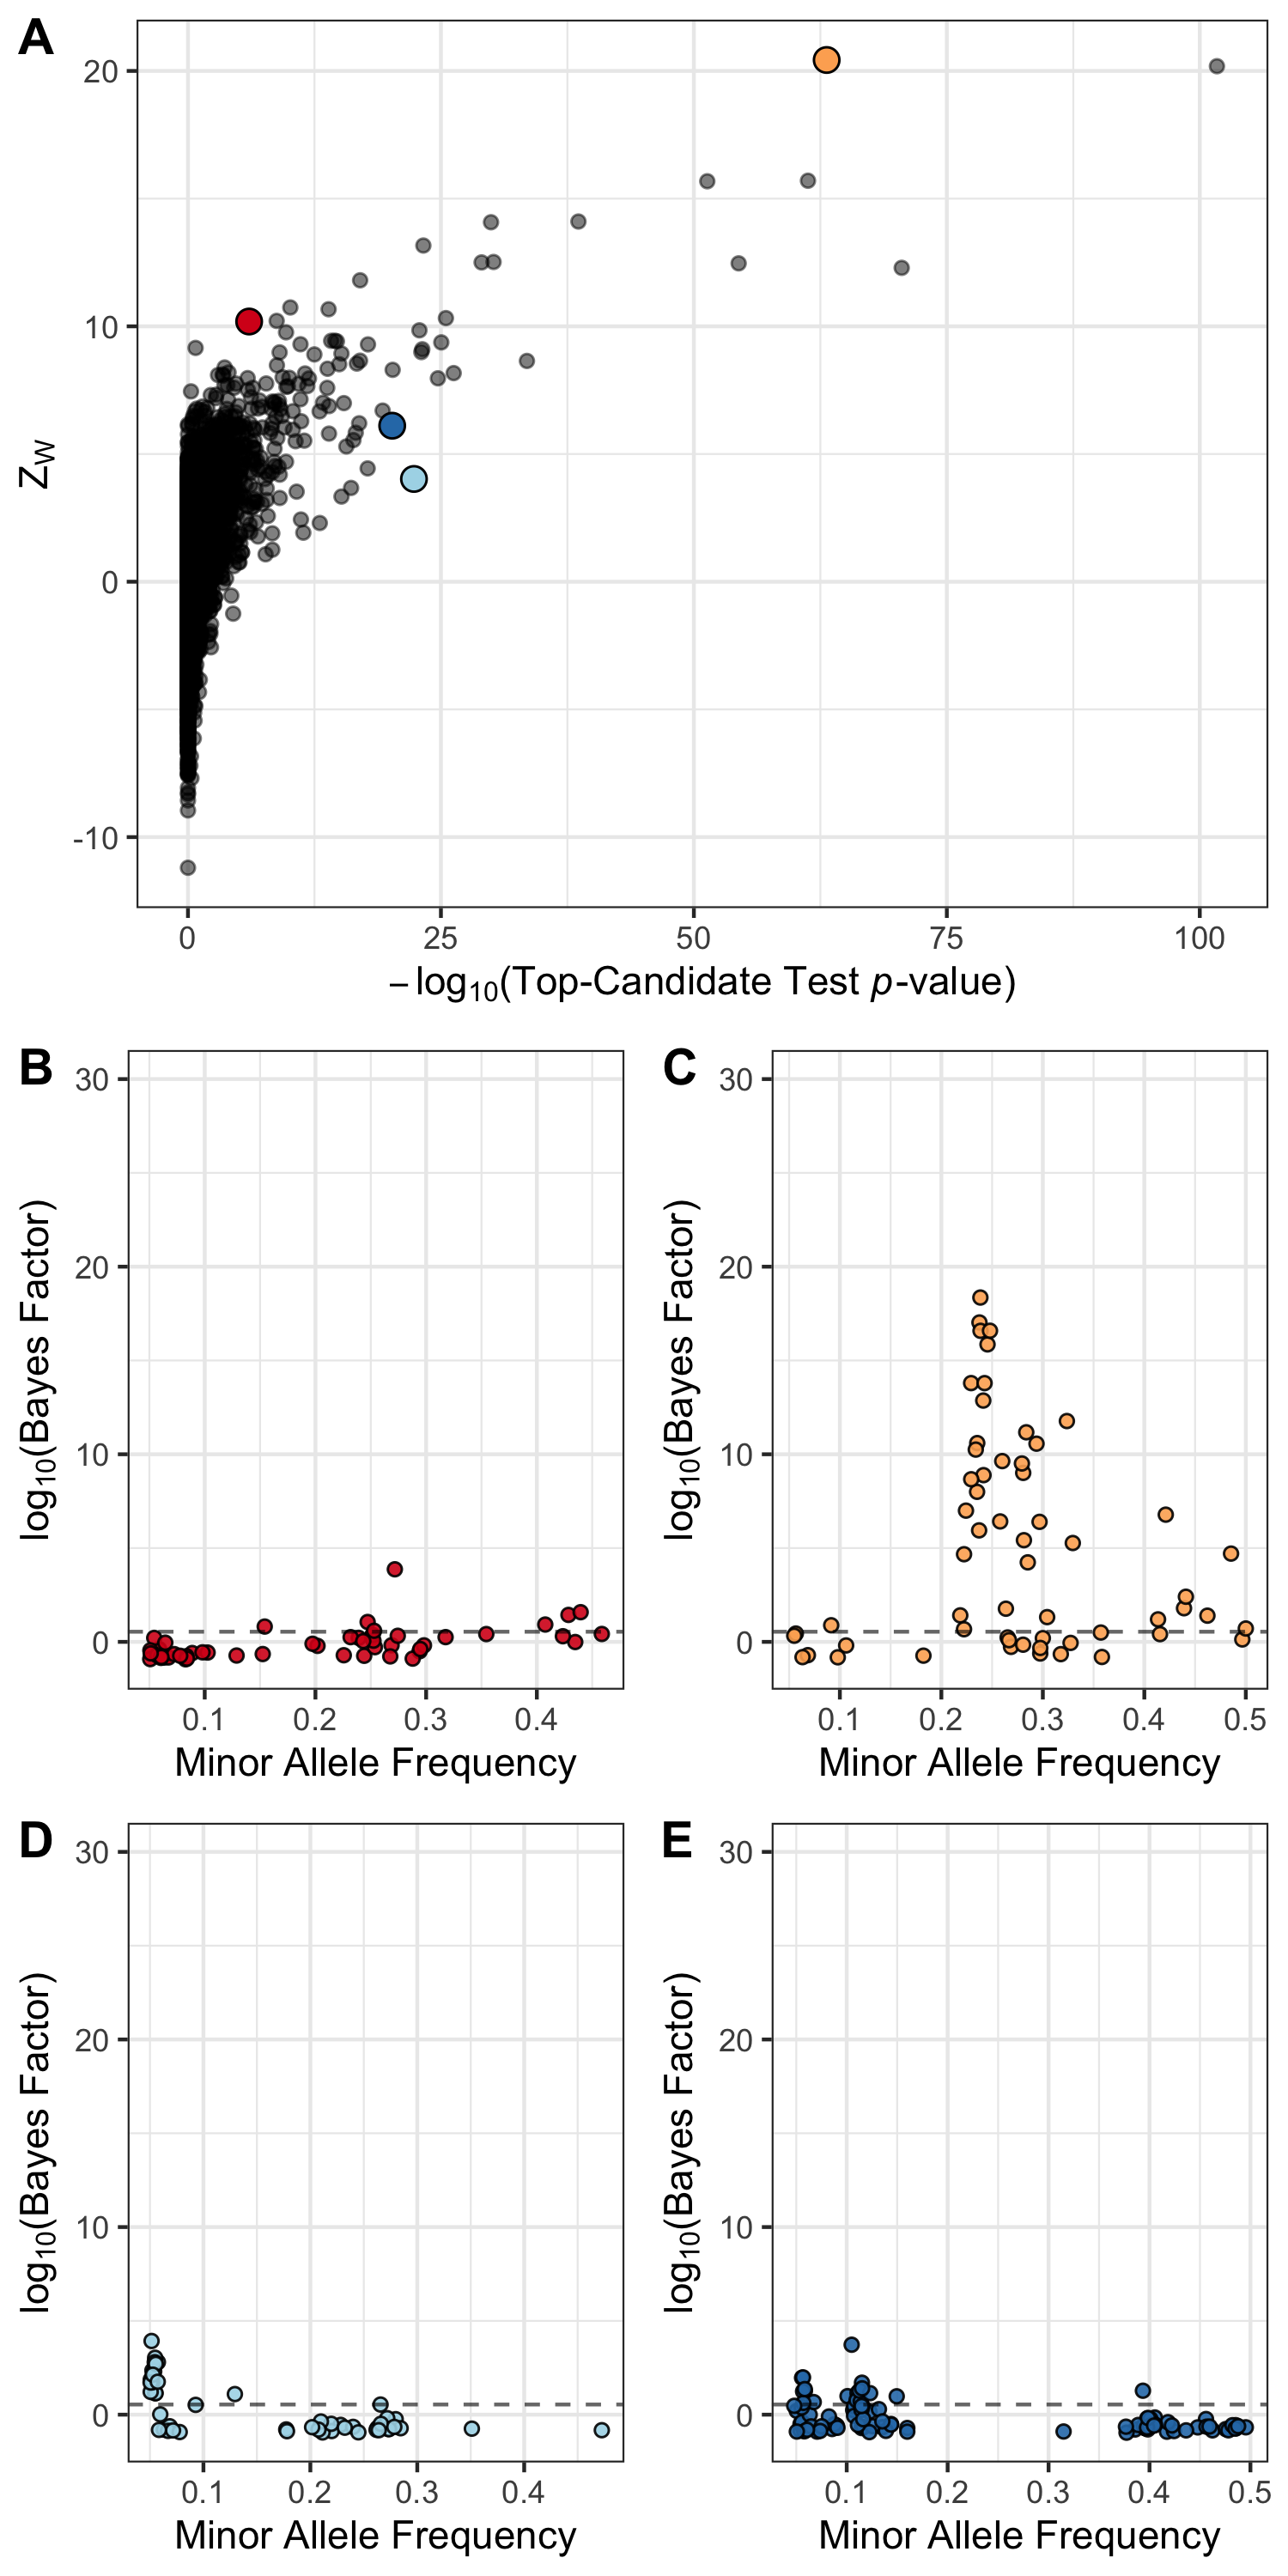
\includegraphics[width=0.75\textwidth,height=0.75\textheight,keepaspectratio]{../dataAnalsis/Z_v_MAF_DD0.png}
  \caption{The WZA applied to GEA results Lodgepole Pine for degree days below 0 (DD0). A) $Z_w$ scores compared to scores from the top-candidate test for each of the genes analyesd by Yeaman et al (2016). Panels B-E show the results for $-log_{10}$(\textit{p}-values) for Spearman's $\rho$ applied to individual SNPs against minor allele frequency (MAF). The dashed horizontal line in B-D indicates the $99^{th}$ percentile of GEA $-log_{10}$(\textit{p}-values) genome-wide.}

  \label{fig:lodgepole}
\end{figure}


\section{Discussion}

Genomic regions of low recombination exhibit greater variance in population genetic summary statistics than do more highly recombining ones, complicating statistical inference. We simulated genomes that experience uniform recombination rates, though that is highly unrealistic. We did so for statistical convenience. When analysing real datasets, researchers should be mindful that analysis windows of a constant physical size may generate statistical artefacts as we outlined in our previous study (Booker et al 2020).

Paragraph about weak selection...
Populations may be adapted to 



There are philosophical reasons as to why the WZA should be preferred. First, the top-candidate test assumes that there is a fraction of the genetic markers analysed that are tagging causal variants (i.e. that there are true positives in the dataset). This is undesirable, because there may well be no detectable variation that contributes to local adaptation present, i.e. genuine genotype-environment correlations may be very weak and the study are simply underpowered. Secondly, the top-candidate test gives equal weight to all markers. However, alleles at different frequencies possess different levels of information about population history. A final related point is that all SNPs that have exceeded the significance threshold are treated identically. For example, with a significance threshold of 0.01, genomic regions with only a single outlier are treated in the same way whether that outlier has a \textit{p}-value of 0.009 or $10^{-10}$.


\section{Acknowledgements}

Thanks to Pooja Singh for discussions, to Tongli Wang for help with BC climate data and to Simon Kapitza for help with wrangling raster files. 


\section{Bibliography}


%\bibliography{example-bibliography}


\section{Appendix}


Consider a hypothetical metapopulation of 1 million individuals distributed evenly among 196 demes. It would be computationally intractable to simulate all $10^6$ individuals forward-in-time, incorporating adaptation to environmental heterogeneity across a landscape and recombining chromosomes. We scaled several population genetic parameters to model a large population by simulating a much smaller population. In the following sections, we outline and justify the approach we used to scale pertinent population genetic parameters. 

\subsubsection{Recombination rates}

In panmictic populations, linkage disequilibrium can be predicted by the scaled recombination parameter $\rho = 4N_er$, where \textit{r} is the recombination rate per base-pair and $N_e$ is the effective population size. In structured populations, LD is elevated above the panmictic expectation and can be described by the effective size of the local population (or deme), the recombination rate and the migration rate (McVean paper). Assuming a recombination rate of 1 cM/Mbp, the hypothetical organism would have $4N_dr = 0.0002$. To achieve levels of LD-decay in our simulations that are similar to those expected in our hypothetical organism, we set $4N_dr = 0.0002$, but with only 100 individuals per deme that gave a per base pair recombination of $5.10 \times 10^{-7}$.

\subsubsection{Selection coefficients} 

It is difficult to choose a realistic set of selection parameters for modelling local adaptation because there are, at present, few estimates of the distribution of fitness effects for mutations that have spatially divergent effects. However, common garden studies of a variety of taxa have estimated fitness differences of up to 50\% between populations grown in home-like conditions versus away-like conditions (REF). Motivated by such studies, we chose to parameterise selection using the maximum possible fitness difference between home versus away environments. By setting the maximum reduction to $!$
have demonstrated in a variety of taxa that there 

\subsubsection{Migration rate} 

For the migration rate, we worked backwards. We set out to achieve $F_{ST}$ across the metapopulation of around 0.05, as has been reported for a numerous widely distributed tree species (REF). For an island model, we can 

\subsubsection{Mutation rate} 


\begin{table}[]
\label{SimulationParameters}
\caption{Population genetic parameters of a hypothetical organism, and how they are scaled in the simulations. The meta-population inhabits a $14\times14$ 2-dimensional stepping stone. Parameters are shown for a population with 10 loci subject to directional selection.}
\begin{tabular}{lcccl}
\cline{1-4}
\textbf{Parameter} & \textbf{Biological Value} & \textbf{Scaled Parameter}        & \textbf{Unscaled (simulation)} \\ \cline{1-4}
Global population size ($N_e$)                 & $10^6$                                      & -                           & 19,600                                              &           \\
Number of demes ($d$)                  & 196                                      & -                           & 196                                                &           \\
Local population size ($N_d$)                  & 5,100                                      & -                           & 100                                                &           \\
Recombination rate (\textit{r})                        & $10^{-8}$                                      & $4N_dr = 2.04 \times 10^{-4}$ & $5.10 \times 10^{-7}$                                           &           \\
Selection coefficient (\textit{$s_{Max}$})                        & 0.005                                         & $2N_ds_{Max}= 25.5$ & 0.255                                           &           \\
Migration rate (\textit{m})                        & $9.80\times 10^{-4}$                                      & $2N_dm = 10$        & 0.05                                               &           \\
Functional mutation rate (\textit{$\mu_\alpha$})                        & $2\times 10^{-10}$                                      & $4N_e\mu_\alpha = 0.0008$        & $10^{-8}$ &           \\ \cline{1-4}
\end{tabular}
\end{table}
\subsubsection{Chromosomal architecture}


\begin{figure}
  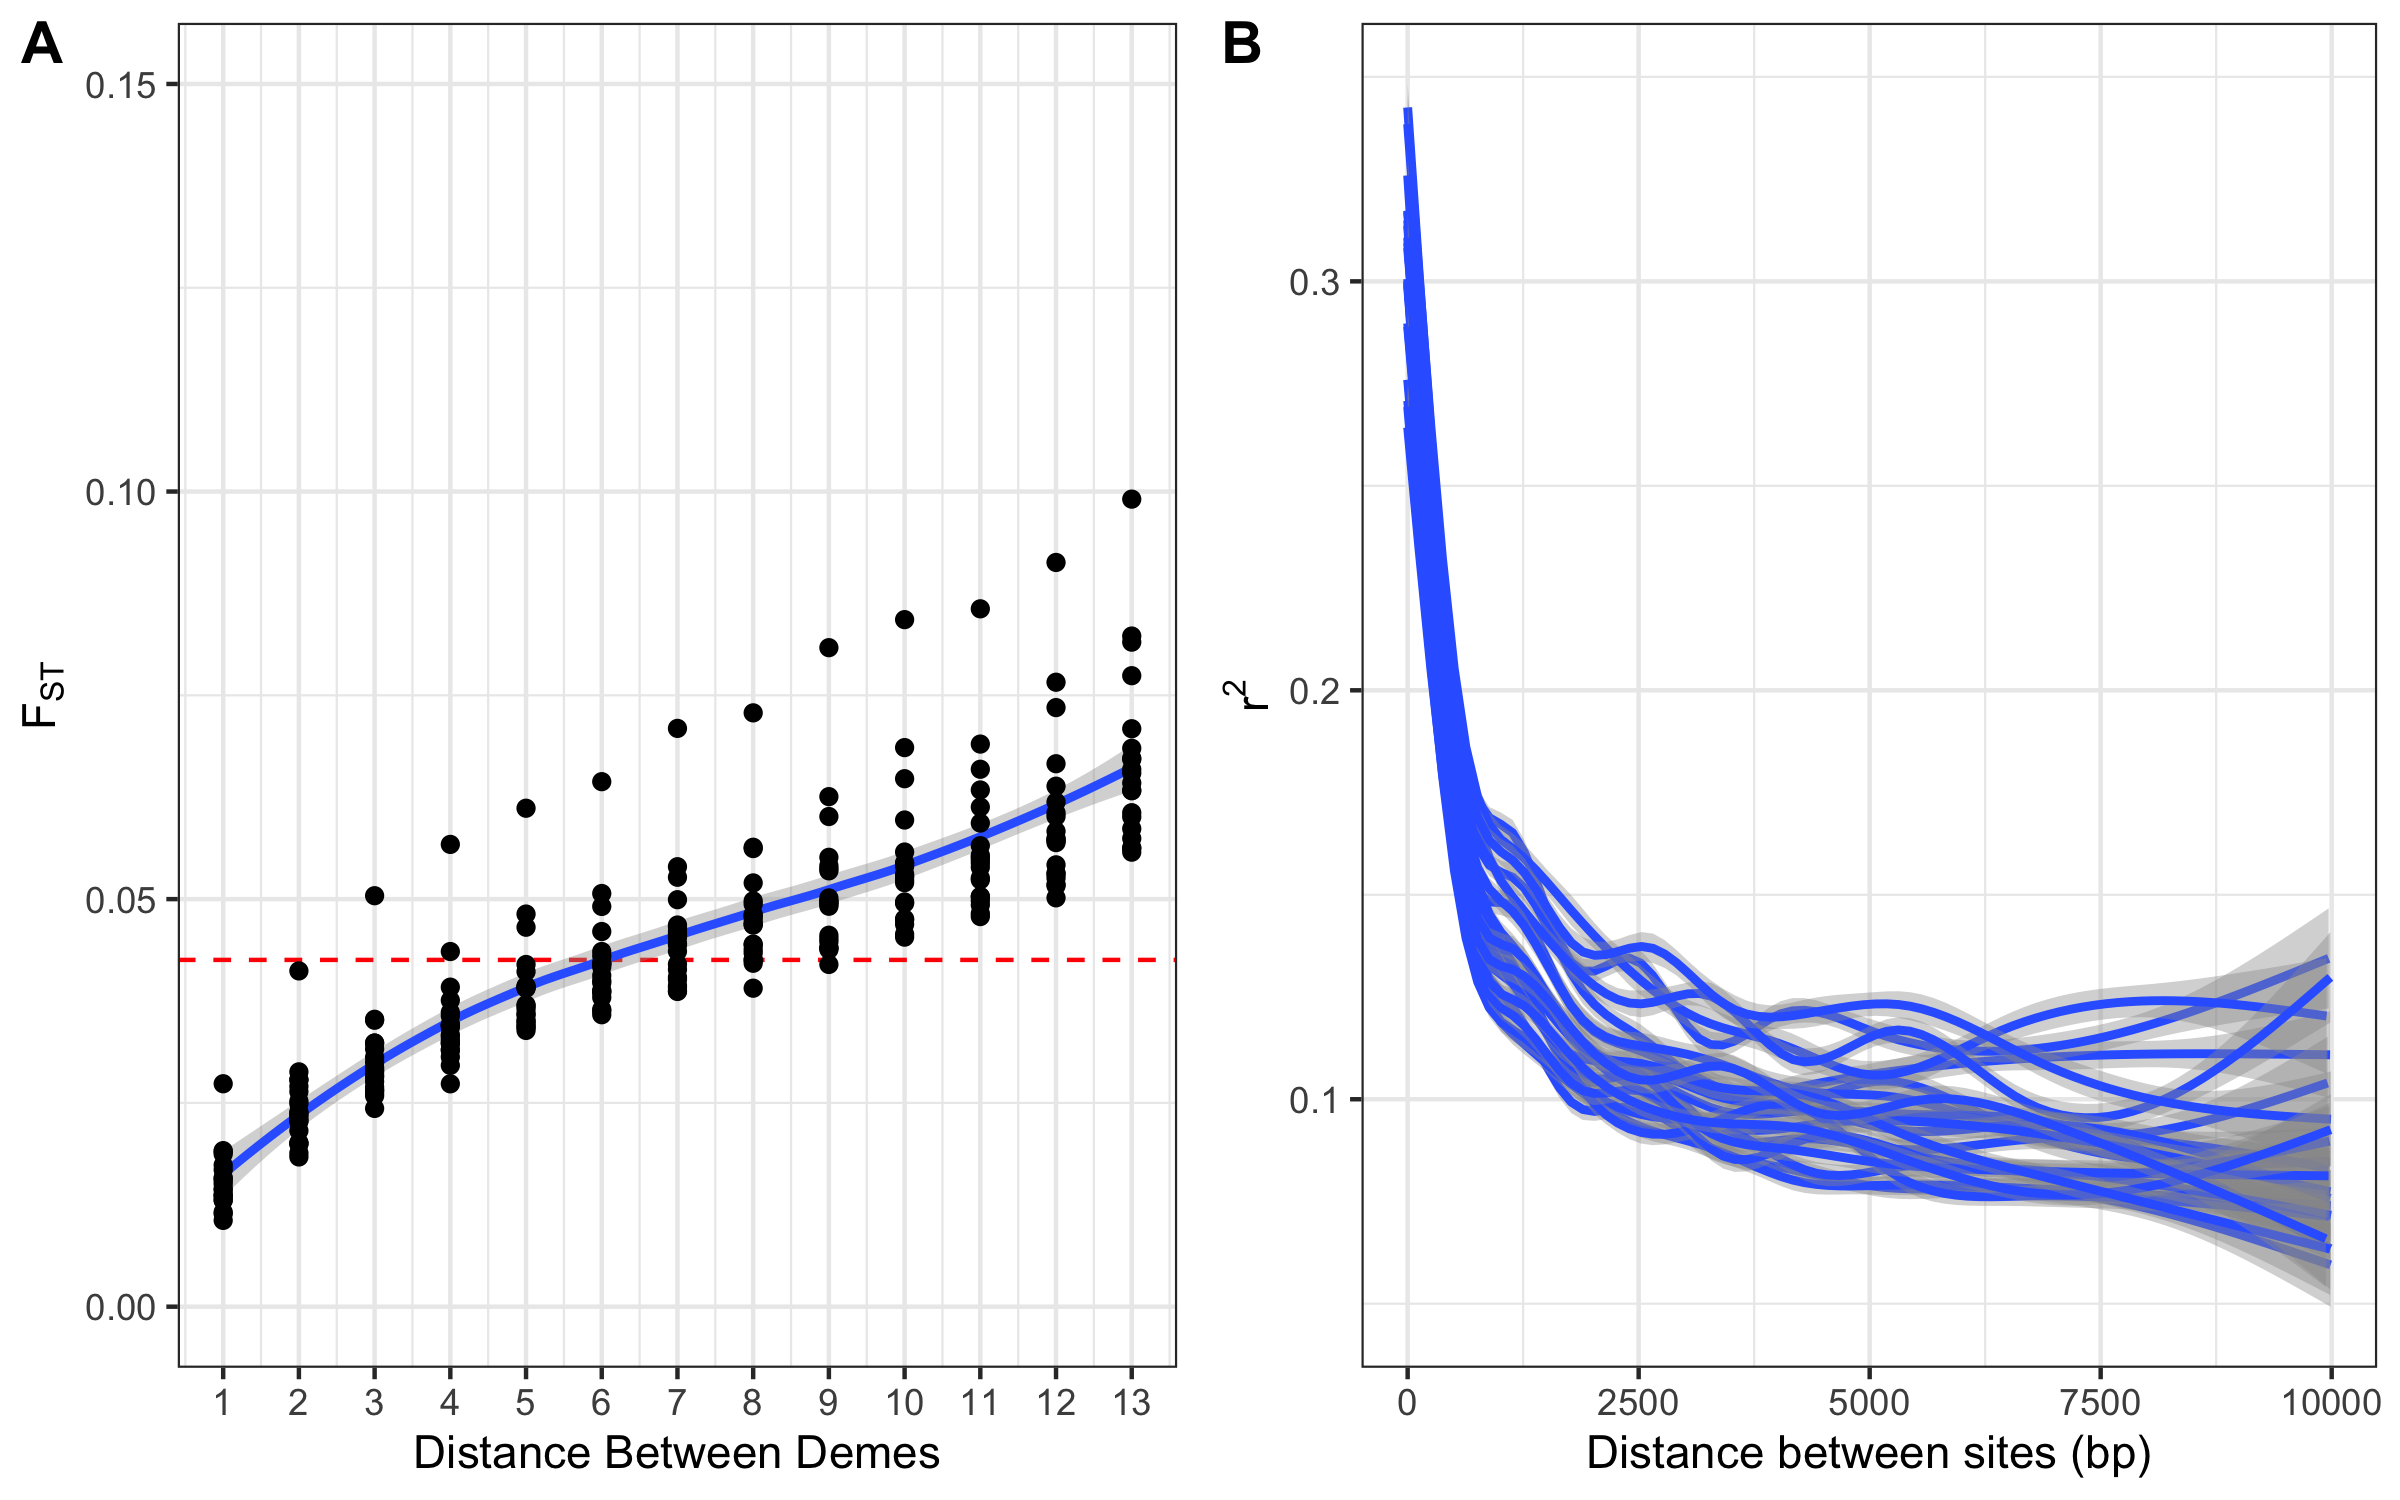
\includegraphics[width=0.75\textwidth,height=0.75\textheight,keepaspectratio]{../SimulationStudy/directionalSelection/SummaryStats.png}
  \caption{Summary statistics from simulations. A) shows the $F_{ST}$ between pairs of demes in stepping-stone populations, the average across replicates is . B) shows the average LD between pairs of SNPs, each line corresponds to a single simulation replicate.}

  \label{fig:lodgepole}
\end{figure}


\end{document}